% !TEX root = document.tex
% =====================================================================
% 第4章 图形界面使用方法 —— 界面型软件的核心章，命令行软件可整章删掉
%
% 写什么（按顺序走一遍界面，像带人操作）：
%   1. 启动与登录：怎么打开、有没有登录。
%   2. 主界面：整体布局，放一张全屏截图。
%   3. 各功能模块：每个页面/按钮做什么，操作后发生什么，配截图。
%   4. 完整操作流程：从进入软件到拿到结果的连贯步骤。
%
% 截图的硬要求（审查重点）：
%   - 提供一张完整界面图建立整体印象，再用局部操作图说明关键步骤。
%   - 截图上的软件名称必须和申请表上的软件名称一致。
%   - 文字与截图要连贯：能看出页面怎么跳转、按了哪个按钮出现哪个界面。
%   - 图片放 images/ 目录，用 \includegraphics，宽度用 0.9\textwidth 之类。
%   - 图要清晰，太大就缩小，可用 subfigure 并排。
%
% 本章是示范文字，images/gui_home.png 为界面示意图，请替换为你的软件真实截图。完整界面图与局部操作图结合即可，不强制每张全屏。
% =====================================================================

\section{图形界面使用方法}
\label{sec:gui_usage}

本章以浏览器界面为例说明\Name{}的操作方式。界面与命令行共用同一套处理逻辑，两种方式的结果一致。

\subsection{启动与进入}
\label{ssec:gui_start}
按第\ref{sec:installation}章的命令启动服务后，在浏览器打开\url{http://localhost:8501}，进入软件首页。首页顶部显示软件名称，与申请表登记的名称一致。

\begin{figure}[!h]
\centering
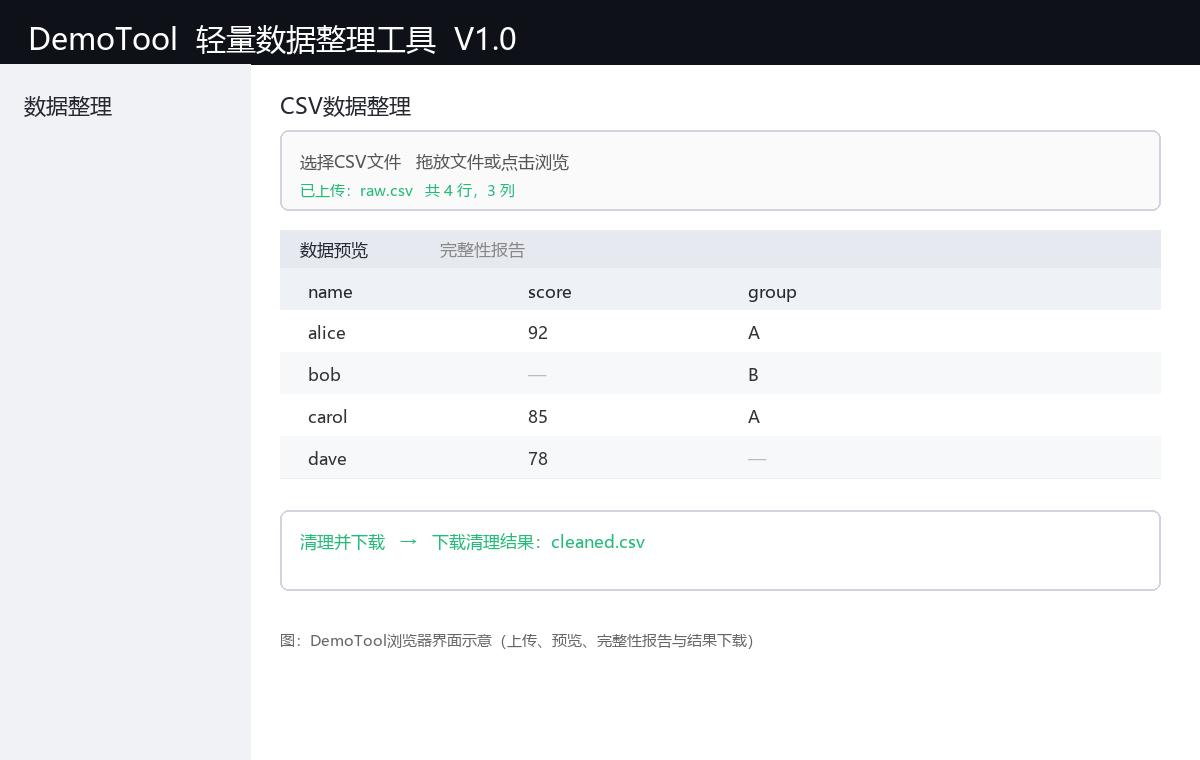
\includegraphics[width=0.9\textwidth]{images/gui_home.png}
\caption{\Name{}浏览器界面：上传、预览、报告与下载}
\label{fig:gui_home}
\end{figure}

\subsection{数据上传与预览}
\label{ssec:gui_upload}
在首页的"选择CSV文件"区域点击上传按钮，选取本地CSV文件。上传后页面显示数据行数与列数，并在"数据预览"标签页列出前20行。用户可在上传新文件替换当前数据。

上传与预览区域见前面\ref{fig:gui_home}的界面示意图。

\subsection{完整性报告}
\label{ssec:gui_report}
切换到"完整性报告"标签页，页面以表格形式列出每一列的总数、非空数、缺失数与不同值个数。缺失数由总数与非空数之差得到，用于判断哪些列需要先行清理。

\subsection{清理与下载}
\label{ssec:gui_clean}
点击页面下方的"清理并下载"按钮，软件对当前数据执行列名规范化、空白清理与空行过滤，生成\lstinline|cleaned.csv|。点击"下载清理结果"即可保存到本地。按钮所在界面见\ref{fig:gui_home}，操作结果在按钮下方给出下载入口。

\subsection{完整操作流程}
\label{ssec:gui_flow}
一次典型的界面操作按以下顺序进行：
\begin{enumerate}
    \item 启动服务并进入首页；
    \item 上传待整理的CSV文件；
    \item 在"数据预览"中确认文件内容与列结构；
    \item 在"完整性报告"中查看各列缺失情况；
    \item 点击"清理并下载"，保存结果文件。
\end{enumerate}
每一步对应的界面截图见前述各节。页面之间的跳转由标签页切换和按钮点击触发，截图与文字按顺序对应。
